\documentclass[twoside]{book}

% Packages required by doxygen
\usepackage{fixltx2e}
\usepackage{calc}
\usepackage{doxygen}
\usepackage[export]{adjustbox} % also loads graphicx
\usepackage{graphicx}
\usepackage[utf8]{inputenc}
\usepackage{makeidx}
\usepackage{multicol}
\usepackage{multirow}
\PassOptionsToPackage{warn}{textcomp}
\usepackage{textcomp}
\usepackage[nointegrals]{wasysym}
\usepackage[table]{xcolor}

% Font selection
\usepackage[T1]{fontenc}
\usepackage[scaled=.90]{helvet}
\usepackage{courier}
\usepackage{amssymb}
\usepackage{sectsty}
\renewcommand{\familydefault}{\sfdefault}
\allsectionsfont{%
  \fontseries{bc}\selectfont%
  \color{darkgray}%
}
\renewcommand{\DoxyLabelFont}{%
  \fontseries{bc}\selectfont%
  \color{darkgray}%
}
\newcommand{\+}{\discretionary{\mbox{\scriptsize$\hookleftarrow$}}{}{}}

% Page & text layout
\usepackage{geometry}
\geometry{%
  a4paper,%
  top=2.5cm,%
  bottom=2.5cm,%
  left=2.5cm,%
  right=2.5cm%
}
\tolerance=750
\hfuzz=15pt
\hbadness=750
\setlength{\emergencystretch}{15pt}
\setlength{\parindent}{0cm}
\setlength{\parskip}{3ex plus 2ex minus 2ex}
\makeatletter
\renewcommand{\paragraph}{%
  \@startsection{paragraph}{4}{0ex}{-1.0ex}{1.0ex}{%
    \normalfont\normalsize\bfseries\SS@parafont%
  }%
}
\renewcommand{\subparagraph}{%
  \@startsection{subparagraph}{5}{0ex}{-1.0ex}{1.0ex}{%
    \normalfont\normalsize\bfseries\SS@subparafont%
  }%
}
\makeatother

% Headers & footers
\usepackage{fancyhdr}
\pagestyle{fancyplain}
\fancyhead[LE]{\fancyplain{}{\bfseries\thepage}}
\fancyhead[CE]{\fancyplain{}{}}
\fancyhead[RE]{\fancyplain{}{\bfseries\leftmark}}
\fancyhead[LO]{\fancyplain{}{\bfseries\rightmark}}
\fancyhead[CO]{\fancyplain{}{}}
\fancyhead[RO]{\fancyplain{}{\bfseries\thepage}}
\fancyfoot[LE]{\fancyplain{}{}}
\fancyfoot[CE]{\fancyplain{}{}}
\fancyfoot[RE]{\fancyplain{}{\bfseries\scriptsize Generated by Doxygen }}
\fancyfoot[LO]{\fancyplain{}{\bfseries\scriptsize Generated by Doxygen }}
\fancyfoot[CO]{\fancyplain{}{}}
\fancyfoot[RO]{\fancyplain{}{}}
\renewcommand{\footrulewidth}{0.4pt}
\renewcommand{\chaptermark}[1]{%
  \markboth{#1}{}%
}
\renewcommand{\sectionmark}[1]{%
  \markright{\thesection\ #1}%
}

% Indices & bibliography
\usepackage{natbib}
\usepackage[titles]{tocloft}
\setcounter{tocdepth}{3}
\setcounter{secnumdepth}{5}
\makeindex

% Hyperlinks (required, but should be loaded last)
\usepackage{ifpdf}
\ifpdf
  \usepackage[pdftex,pagebackref=true]{hyperref}
\else
  \usepackage[ps2pdf,pagebackref=true]{hyperref}
\fi
\hypersetup{%
  colorlinks=true,%
  linkcolor=blue,%
  citecolor=blue,%
  unicode%
}

% Custom commands
\newcommand{\clearemptydoublepage}{%
  \newpage{\pagestyle{empty}\cleardoublepage}%
}

\usepackage{caption}
\captionsetup{labelsep=space,justification=centering,font={bf},singlelinecheck=off,skip=4pt,position=top}

%===== C O N T E N T S =====

\begin{document}

% Titlepage & ToC
\hypersetup{pageanchor=false,
             bookmarksnumbered=true,
             pdfencoding=unicode
            }
\pagenumbering{roman}
\begin{titlepage}
\vspace*{7cm}
\begin{center}%
{\Large Calculator }\\
\vspace*{1cm}
{\large Generated by Doxygen 1.8.11}\\
\end{center}
\end{titlepage}
\clearemptydoublepage
\tableofcontents
\clearemptydoublepage
\pagenumbering{arabic}
\hypersetup{pageanchor=true}

%--- Begin generated contents ---
\chapter{Namespace Index}
\section{Packages}
Here are the packages with brief descriptions (if available)\+:\begin{DoxyCompactList}
\item\contentsline{section}{\hyperlink{namespace_calculator}{Calculator} \\*kalkulacka }{\pageref{namespace_calculator}}{}
\end{DoxyCompactList}

\chapter{Hierarchical Index}
\section{Class Hierarchy}
This inheritance list is sorted roughly, but not completely, alphabetically\+:\begin{DoxyCompactList}
\item Form\begin{DoxyCompactList}
\item \contentsline{section}{Calculator.\+Form1}{\pageref{class_calculator_1_1_form1}}{}
\end{DoxyCompactList}
\item \contentsline{section}{Calculator.\+Form1.\+globs}{\pageref{class_calculator_1_1_form1_1_1globs}}{}
\end{DoxyCompactList}

\chapter{Class Index}
\section{Class List}
Here are the classes, structs, unions and interfaces with brief descriptions\+:\begin{DoxyCompactList}
\item\contentsline{section}{\hyperlink{class_calculator_1_1_form1}{Calculator.\+Form1} \\*deklarace kalkulacky }{\pageref{class_calculator_1_1_form1}}{}
\item\contentsline{section}{\hyperlink{class_calculator_1_1_form1_1_1globs}{Calculator.\+Form1.\+globs} \\*cela trida pro pole operandu a cisel }{\pageref{class_calculator_1_1_form1_1_1globs}}{}
\end{DoxyCompactList}

\chapter{Namespace Documentation}
\hypertarget{namespace_calculator}{}\section{Calculator Namespace Reference}
\label{namespace_calculator}\index{Calculator@{Calculator}}


kalkulacka  


\subsection*{Classes}
\begin{DoxyCompactItemize}
\item 
class \hyperlink{class_calculator_1_1_form1}{Form1}
\begin{DoxyCompactList}\small\item\em deklarace kalkulacky \end{DoxyCompactList}\item 
class {\bfseries Program}
\begin{DoxyCompactList}\small\item\em deklarace gui \end{DoxyCompactList}\end{DoxyCompactItemize}


\subsection{Detailed Description}
kalkulacka 


\chapter{Class Documentation}
\hypertarget{class_calculator_1_1_form1}{}\section{Calculator.\+Form1 Class Reference}
\label{class_calculator_1_1_form1}\index{Calculator.\+Form1@{Calculator.\+Form1}}


deklarace kalkulacky  


Inheritance diagram for Calculator.\+Form1\+:\begin{figure}[H]
\begin{center}
\leavevmode
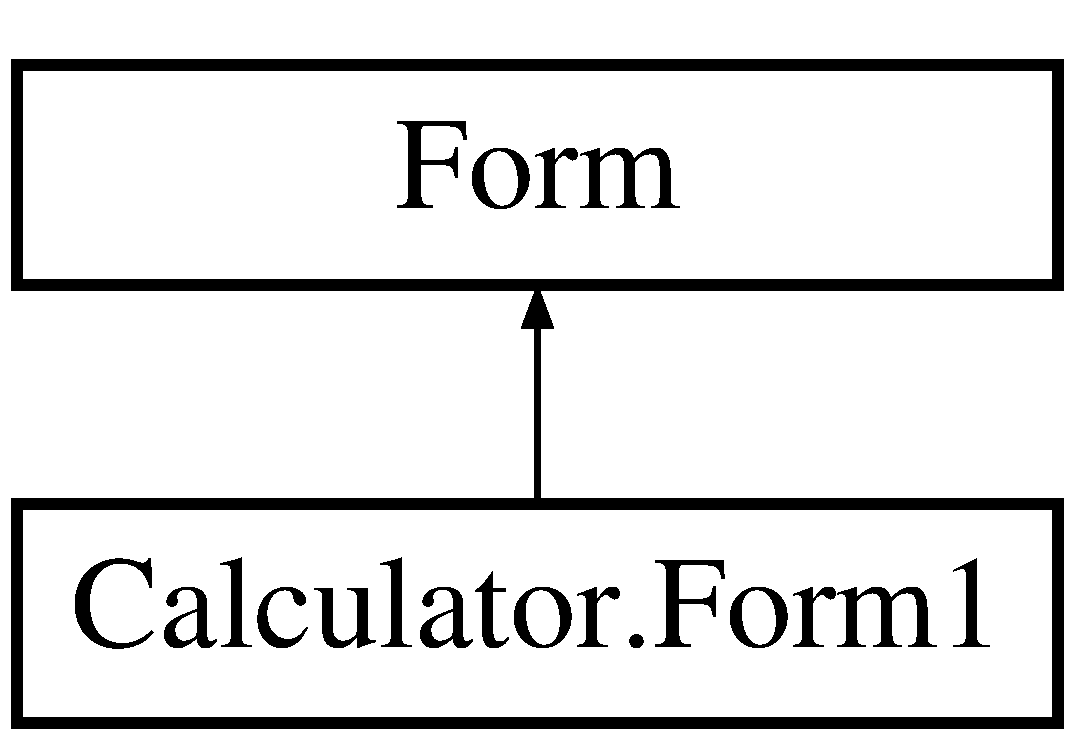
\includegraphics[height=2.000000cm]{class_calculator_1_1_form1}
\end{center}
\end{figure}
\subsection*{Classes}
\begin{DoxyCompactItemize}
\item 
class {\bfseries Globals}
\begin{DoxyCompactList}\small\item\em nastaveni promnenych \end{DoxyCompactList}\item 
class \hyperlink{class_calculator_1_1_form1_1_1globs}{globs}
\begin{DoxyCompactList}\small\item\em cela trida pro pole operandu a cisel \end{DoxyCompactList}\end{DoxyCompactItemize}
\subsection*{Public Member Functions}
\begin{DoxyCompactItemize}
\item 
\hyperlink{class_calculator_1_1_form1_a095b483116463d21326329c5b0427d04}{Form1} ()
\begin{DoxyCompactList}\small\item\em zakladni nastaveni kalkulacky \end{DoxyCompactList}\item 
void \hyperlink{class_calculator_1_1_form1_a1b98650937b3ca663bebdf5956c1d0ee}{add\+Char\+To\+Textbox} (char a)
\begin{DoxyCompactList}\small\item\em kontrola a pridani do znaku textboxu \end{DoxyCompactList}\item 
void \hyperlink{class_calculator_1_1_form1_a5197b700927d7cd8c4408f8a033f6c31}{clear\+Function} ()
\begin{DoxyCompactList}\small\item\em vycisteni celeho pole a textboxu \end{DoxyCompactList}\item 
void \hyperlink{class_calculator_1_1_form1_a0e349ae0eec13af39bd03c97d5f63110}{set\+Value} (int y, float value)
\begin{DoxyCompactList}\small\item\em nastaveni hodnoty pocitanych cisel smazani ostatnich pokud uz byli pouzity \end{DoxyCompactList}\item 
void \hyperlink{class_calculator_1_1_form1_a77b79cdc88b91b57427780d80d8e2f74}{equals\+Function} ()
\begin{DoxyCompactList}\small\item\em nastaveni vstupu z klavesnice \end{DoxyCompactList}\item 
void \hyperlink{class_calculator_1_1_form1_ad9f716fe86d8d2d03a50f93488f52368}{set\+Operator} (char op)
\begin{DoxyCompactList}\small\item\em nastaveni operatoru \end{DoxyCompactList}\item 
void \hyperlink{class_calculator_1_1_form1_a6b3fab065d9c21db2311ddfac505ba7e}{set\+Things} ()
\begin{DoxyCompactList}\small\item\em potvrzeni pro zadani operatoru a moznost zaporneho cisla \end{DoxyCompactList}\item 
void \hyperlink{class_calculator_1_1_form1_a8517e0865c2b1cba341f7d8f2eec4a3d}{set\+Defaults} ()
\begin{DoxyCompactList}\small\item\em nastaveni vychoziho stavu \end{DoxyCompactList}\end{DoxyCompactItemize}
\subsection*{Protected Member Functions}
\begin{DoxyCompactItemize}
\item 
override void \hyperlink{class_calculator_1_1_form1_a0dc657efe9d8fed0e1a50cc4af2214e8}{Dispose} (bool disposing)
\begin{DoxyCompactList}\small\item\em vycisteni zdroju pred pouzitim \end{DoxyCompactList}\end{DoxyCompactItemize}


\subsection{Detailed Description}
deklarace kalkulacky 

graficke rozhrani 

\subsection{Constructor \& Destructor Documentation}
\index{Calculator\+::\+Form1@{Calculator\+::\+Form1}!Form1@{Form1}}
\index{Form1@{Form1}!Calculator\+::\+Form1@{Calculator\+::\+Form1}}
\subsubsection[{\texorpdfstring{Form1()}{Form1()}}]{\setlength{\rightskip}{0pt plus 5cm}Calculator.\+Form1.\+Form1 (
\begin{DoxyParamCaption}
{}
\end{DoxyParamCaption}
)}\hypertarget{class_calculator_1_1_form1_a095b483116463d21326329c5b0427d04}{}\label{class_calculator_1_1_form1_a095b483116463d21326329c5b0427d04}


zakladni nastaveni kalkulacky 



\subsection{Member Function Documentation}
\index{Calculator\+::\+Form1@{Calculator\+::\+Form1}!add\+Char\+To\+Textbox@{add\+Char\+To\+Textbox}}
\index{add\+Char\+To\+Textbox@{add\+Char\+To\+Textbox}!Calculator\+::\+Form1@{Calculator\+::\+Form1}}
\subsubsection[{\texorpdfstring{add\+Char\+To\+Textbox(char a)}{addCharToTextbox(char a)}}]{\setlength{\rightskip}{0pt plus 5cm}void Calculator.\+Form1.\+add\+Char\+To\+Textbox (
\begin{DoxyParamCaption}
\item[{char}]{a}
\end{DoxyParamCaption}
)}\hypertarget{class_calculator_1_1_form1_a1b98650937b3ca663bebdf5956c1d0ee}{}\label{class_calculator_1_1_form1_a1b98650937b3ca663bebdf5956c1d0ee}


kontrola a pridani do znaku textboxu 


\begin{DoxyParams}{Parameters}
{\em a} & pridavany znak \\
\hline
\end{DoxyParams}
\index{Calculator\+::\+Form1@{Calculator\+::\+Form1}!clear\+Function@{clear\+Function}}
\index{clear\+Function@{clear\+Function}!Calculator\+::\+Form1@{Calculator\+::\+Form1}}
\subsubsection[{\texorpdfstring{clear\+Function()}{clearFunction()}}]{\setlength{\rightskip}{0pt plus 5cm}void Calculator.\+Form1.\+clear\+Function (
\begin{DoxyParamCaption}
{}
\end{DoxyParamCaption}
)}\hypertarget{class_calculator_1_1_form1_a5197b700927d7cd8c4408f8a033f6c31}{}\label{class_calculator_1_1_form1_a5197b700927d7cd8c4408f8a033f6c31}


vycisteni celeho pole a textboxu 

\index{Calculator\+::\+Form1@{Calculator\+::\+Form1}!Dispose@{Dispose}}
\index{Dispose@{Dispose}!Calculator\+::\+Form1@{Calculator\+::\+Form1}}
\subsubsection[{\texorpdfstring{Dispose(bool disposing)}{Dispose(bool disposing)}}]{\setlength{\rightskip}{0pt plus 5cm}override void Calculator.\+Form1.\+Dispose (
\begin{DoxyParamCaption}
\item[{bool}]{disposing}
\end{DoxyParamCaption}
)\hspace{0.3cm}{\ttfamily [protected]}}\hypertarget{class_calculator_1_1_form1_a0dc657efe9d8fed0e1a50cc4af2214e8}{}\label{class_calculator_1_1_form1_a0dc657efe9d8fed0e1a50cc4af2214e8}


vycisteni zdroju pred pouzitim 


\begin{DoxyParams}{Parameters}
{\em disposing} & pravda pokud zdoje mouhou byt pouzity, jinak false \\
\hline
\end{DoxyParams}
\index{Calculator\+::\+Form1@{Calculator\+::\+Form1}!equals\+Function@{equals\+Function}}
\index{equals\+Function@{equals\+Function}!Calculator\+::\+Form1@{Calculator\+::\+Form1}}
\subsubsection[{\texorpdfstring{equals\+Function()}{equalsFunction()}}]{\setlength{\rightskip}{0pt plus 5cm}void Calculator.\+Form1.\+equals\+Function (
\begin{DoxyParamCaption}
{}
\end{DoxyParamCaption}
)}\hypertarget{class_calculator_1_1_form1_a77b79cdc88b91b57427780d80d8e2f74}{}\label{class_calculator_1_1_form1_a77b79cdc88b91b57427780d80d8e2f74}


nastaveni vstupu z klavesnice 

\index{Calculator\+::\+Form1@{Calculator\+::\+Form1}!set\+Defaults@{set\+Defaults}}
\index{set\+Defaults@{set\+Defaults}!Calculator\+::\+Form1@{Calculator\+::\+Form1}}
\subsubsection[{\texorpdfstring{set\+Defaults()}{setDefaults()}}]{\setlength{\rightskip}{0pt plus 5cm}void Calculator.\+Form1.\+set\+Defaults (
\begin{DoxyParamCaption}
{}
\end{DoxyParamCaption}
)}\hypertarget{class_calculator_1_1_form1_a8517e0865c2b1cba341f7d8f2eec4a3d}{}\label{class_calculator_1_1_form1_a8517e0865c2b1cba341f7d8f2eec4a3d}


nastaveni vychoziho stavu 

\index{Calculator\+::\+Form1@{Calculator\+::\+Form1}!set\+Operator@{set\+Operator}}
\index{set\+Operator@{set\+Operator}!Calculator\+::\+Form1@{Calculator\+::\+Form1}}
\subsubsection[{\texorpdfstring{set\+Operator(char op)}{setOperator(char op)}}]{\setlength{\rightskip}{0pt plus 5cm}void Calculator.\+Form1.\+set\+Operator (
\begin{DoxyParamCaption}
\item[{char}]{op}
\end{DoxyParamCaption}
)}\hypertarget{class_calculator_1_1_form1_ad9f716fe86d8d2d03a50f93488f52368}{}\label{class_calculator_1_1_form1_ad9f716fe86d8d2d03a50f93488f52368}


nastaveni operatoru 


\begin{DoxyParams}{Parameters}
{\em op} & hodnota operatoru \\
\hline
\end{DoxyParams}
\index{Calculator\+::\+Form1@{Calculator\+::\+Form1}!set\+Things@{set\+Things}}
\index{set\+Things@{set\+Things}!Calculator\+::\+Form1@{Calculator\+::\+Form1}}
\subsubsection[{\texorpdfstring{set\+Things()}{setThings()}}]{\setlength{\rightskip}{0pt plus 5cm}void Calculator.\+Form1.\+set\+Things (
\begin{DoxyParamCaption}
{}
\end{DoxyParamCaption}
)}\hypertarget{class_calculator_1_1_form1_a6b3fab065d9c21db2311ddfac505ba7e}{}\label{class_calculator_1_1_form1_a6b3fab065d9c21db2311ddfac505ba7e}


potvrzeni pro zadani operatoru a moznost zaporneho cisla 

\index{Calculator\+::\+Form1@{Calculator\+::\+Form1}!set\+Value@{set\+Value}}
\index{set\+Value@{set\+Value}!Calculator\+::\+Form1@{Calculator\+::\+Form1}}
\subsubsection[{\texorpdfstring{set\+Value(int y, float value)}{setValue(int y, float value)}}]{\setlength{\rightskip}{0pt plus 5cm}void Calculator.\+Form1.\+set\+Value (
\begin{DoxyParamCaption}
\item[{int}]{y, }
\item[{float}]{value}
\end{DoxyParamCaption}
)}\hypertarget{class_calculator_1_1_form1_a0e349ae0eec13af39bd03c97d5f63110}{}\label{class_calculator_1_1_form1_a0e349ae0eec13af39bd03c97d5f63110}


nastaveni hodnoty pocitanych cisel smazani ostatnich pokud uz byli pouzity 


\begin{DoxyParams}{Parameters}
{\em y} & pozice prvku ke kteremu se pricita \\
\hline
{\em value} & hodnota, ktera se ulozi do prvku na pozici \textquotesingle{}y\textquotesingle{} \\
\hline
\end{DoxyParams}


The documentation for this class was generated from the following files\+:\begin{DoxyCompactItemize}
\item 
C\+:/\+Users/\+Martin/\+Desktop/pro\+F\+I\+Tguys-\/documentatio/\+Calculator/Form1.\+cs\item 
C\+:/\+Users/\+Martin/\+Desktop/pro\+F\+I\+Tguys-\/documentatio/\+Calculator/Form1.\+Designer.\+cs\end{DoxyCompactItemize}

\hypertarget{class_calculator_1_1_form1_1_1globs}{}\section{Calculator.\+Form1.\+globs Class Reference}
\label{class_calculator_1_1_form1_1_1globs}\index{Calculator.\+Form1.\+globs@{Calculator.\+Form1.\+globs}}


cela trida pro pole operandu a cisel  


\subsection*{Public Member Functions}
\begin{DoxyCompactItemize}
\item 
void \hyperlink{class_calculator_1_1_form1_1_1globs_a13fc976548fe1c162cfb142563ea697a}{add\+Num} (float a)
\begin{DoxyCompactList}\small\item\em napsani cisla do pole \end{DoxyCompactList}\item 
int \hyperlink{class_calculator_1_1_form1_1_1globs_abdbbbadfb7bea7c58f47d27e6cda54b2}{get\+Num\+Size} ()
\begin{DoxyCompactList}\small\item\em získani hodnoty cisla ze vstupu a ulozeni \end{DoxyCompactList}\item 
float \hyperlink{class_calculator_1_1_form1_1_1globs_a0479546e140f7cb46832192804e3efe2}{get\+Num\+Item} (int item)
\begin{DoxyCompactList}\small\item\em pocet prvku v poli \end{DoxyCompactList}\item 
void \hyperlink{class_calculator_1_1_form1_1_1globs_a741e3a2ad3a59a57f9ef9bfdbcb9c340}{set\+Value} (int i, float value)
\begin{DoxyCompactList}\small\item\em prevest cislo na pozadovane pozici vystupni hodnotu \end{DoxyCompactList}\item 
void \hyperlink{class_calculator_1_1_form1_1_1globs_a15f497cf643e75497996caf35aef4034}{add\+Op} (char op)
\begin{DoxyCompactList}\small\item\em pridani hodnoty operandu \end{DoxyCompactList}\item 
int \hyperlink{class_calculator_1_1_form1_1_1globs_a6df5edeb5ac1cbe4a8096e7ddaf05791}{get\+Op\+Size} ()
\begin{DoxyCompactList}\small\item\em ziskani hodnoty operandu \end{DoxyCompactList}\item 
char \hyperlink{class_calculator_1_1_form1_1_1globs_a296cd6655c68e7dd9b3a179fa835658e}{get\+Op\+Item} (int item)
\begin{DoxyCompactList}\small\item\em vraceni pozadovaneho operandu s hodnotou item \end{DoxyCompactList}\end{DoxyCompactItemize}
\subsection*{Public Attributes}
\begin{DoxyCompactItemize}
\item 
List$<$ float $>$ \hyperlink{class_calculator_1_1_form1_1_1globs_a43533d815e869c1c69a675663a553cc7}{numbers} = new List$<$float$>$()
\begin{DoxyCompactList}\small\item\em pole cisel \end{DoxyCompactList}\item 
List$<$ char $>$ \hyperlink{class_calculator_1_1_form1_1_1globs_a801693dfdbcc3eab7b9732224c021895}{operands} = new List$<$char$>$()
\begin{DoxyCompactList}\small\item\em pole operandu \end{DoxyCompactList}\end{DoxyCompactItemize}


\subsection{Detailed Description}
cela trida pro pole operandu a cisel 



\subsection{Member Function Documentation}
\index{Calculator\+::\+Form1\+::globs@{Calculator\+::\+Form1\+::globs}!add\+Num@{add\+Num}}
\index{add\+Num@{add\+Num}!Calculator\+::\+Form1\+::globs@{Calculator\+::\+Form1\+::globs}}
\subsubsection[{\texorpdfstring{add\+Num(float a)}{addNum(float a)}}]{\setlength{\rightskip}{0pt plus 5cm}void Calculator.\+Form1.\+globs.\+add\+Num (
\begin{DoxyParamCaption}
\item[{float}]{a}
\end{DoxyParamCaption}
)}\hypertarget{class_calculator_1_1_form1_1_1globs_a13fc976548fe1c162cfb142563ea697a}{}\label{class_calculator_1_1_form1_1_1globs_a13fc976548fe1c162cfb142563ea697a}


napsani cisla do pole 


\begin{DoxyParams}{Parameters}
{\em a} & napsani prvniho cisla ze vstupu \\
\hline
\end{DoxyParams}
\index{Calculator\+::\+Form1\+::globs@{Calculator\+::\+Form1\+::globs}!add\+Op@{add\+Op}}
\index{add\+Op@{add\+Op}!Calculator\+::\+Form1\+::globs@{Calculator\+::\+Form1\+::globs}}
\subsubsection[{\texorpdfstring{add\+Op(char op)}{addOp(char op)}}]{\setlength{\rightskip}{0pt plus 5cm}void Calculator.\+Form1.\+globs.\+add\+Op (
\begin{DoxyParamCaption}
\item[{char}]{op}
\end{DoxyParamCaption}
)}\hypertarget{class_calculator_1_1_form1_1_1globs_a15f497cf643e75497996caf35aef4034}{}\label{class_calculator_1_1_form1_1_1globs_a15f497cf643e75497996caf35aef4034}


pridani hodnoty operandu 


\begin{DoxyParams}{Parameters}
{\em op} & hodnoa operandu \\
\hline
\end{DoxyParams}
\index{Calculator\+::\+Form1\+::globs@{Calculator\+::\+Form1\+::globs}!get\+Num\+Item@{get\+Num\+Item}}
\index{get\+Num\+Item@{get\+Num\+Item}!Calculator\+::\+Form1\+::globs@{Calculator\+::\+Form1\+::globs}}
\subsubsection[{\texorpdfstring{get\+Num\+Item(int item)}{getNumItem(int item)}}]{\setlength{\rightskip}{0pt plus 5cm}float Calculator.\+Form1.\+globs.\+get\+Num\+Item (
\begin{DoxyParamCaption}
\item[{int}]{item}
\end{DoxyParamCaption}
)}\hypertarget{class_calculator_1_1_form1_1_1globs_a0479546e140f7cb46832192804e3efe2}{}\label{class_calculator_1_1_form1_1_1globs_a0479546e140f7cb46832192804e3efe2}


pocet prvku v poli 


\begin{DoxyParams}{Parameters}
{\em item} & pozice prvku v poli \\
\hline
\end{DoxyParams}


\begin{DoxyReturn}{Returns}
hodnota prvku v poli na pozadovane pozici 
\end{DoxyReturn}
\index{Calculator\+::\+Form1\+::globs@{Calculator\+::\+Form1\+::globs}!get\+Num\+Size@{get\+Num\+Size}}
\index{get\+Num\+Size@{get\+Num\+Size}!Calculator\+::\+Form1\+::globs@{Calculator\+::\+Form1\+::globs}}
\subsubsection[{\texorpdfstring{get\+Num\+Size()}{getNumSize()}}]{\setlength{\rightskip}{0pt plus 5cm}int Calculator.\+Form1.\+globs.\+get\+Num\+Size (
\begin{DoxyParamCaption}
{}
\end{DoxyParamCaption}
)}\hypertarget{class_calculator_1_1_form1_1_1globs_abdbbbadfb7bea7c58f47d27e6cda54b2}{}\label{class_calculator_1_1_form1_1_1globs_abdbbbadfb7bea7c58f47d27e6cda54b2}


získani hodnoty cisla ze vstupu a ulozeni 

\begin{DoxyReturn}{Returns}
hodnotra cisla ze vstupu 
\end{DoxyReturn}
\index{Calculator\+::\+Form1\+::globs@{Calculator\+::\+Form1\+::globs}!get\+Op\+Item@{get\+Op\+Item}}
\index{get\+Op\+Item@{get\+Op\+Item}!Calculator\+::\+Form1\+::globs@{Calculator\+::\+Form1\+::globs}}
\subsubsection[{\texorpdfstring{get\+Op\+Item(int item)}{getOpItem(int item)}}]{\setlength{\rightskip}{0pt plus 5cm}char Calculator.\+Form1.\+globs.\+get\+Op\+Item (
\begin{DoxyParamCaption}
\item[{int}]{item}
\end{DoxyParamCaption}
)}\hypertarget{class_calculator_1_1_form1_1_1globs_a296cd6655c68e7dd9b3a179fa835658e}{}\label{class_calculator_1_1_form1_1_1globs_a296cd6655c68e7dd9b3a179fa835658e}


vraceni pozadovaneho operandu s hodnotou item 


\begin{DoxyParams}{Parameters}
{\em item} & hodnota parametru pro operand \\
\hline
\end{DoxyParams}


\begin{DoxyReturn}{Returns}
$<$ operand na pozici item $>$
\end{DoxyReturn}
\index{Calculator\+::\+Form1\+::globs@{Calculator\+::\+Form1\+::globs}!get\+Op\+Size@{get\+Op\+Size}}
\index{get\+Op\+Size@{get\+Op\+Size}!Calculator\+::\+Form1\+::globs@{Calculator\+::\+Form1\+::globs}}
\subsubsection[{\texorpdfstring{get\+Op\+Size()}{getOpSize()}}]{\setlength{\rightskip}{0pt plus 5cm}int Calculator.\+Form1.\+globs.\+get\+Op\+Size (
\begin{DoxyParamCaption}
{}
\end{DoxyParamCaption}
)}\hypertarget{class_calculator_1_1_form1_1_1globs_a6df5edeb5ac1cbe4a8096e7ddaf05791}{}\label{class_calculator_1_1_form1_1_1globs_a6df5edeb5ac1cbe4a8096e7ddaf05791}


ziskani hodnoty operandu 

\begin{DoxyReturn}{Returns}
hodnota operandu 
\end{DoxyReturn}
\index{Calculator\+::\+Form1\+::globs@{Calculator\+::\+Form1\+::globs}!set\+Value@{set\+Value}}
\index{set\+Value@{set\+Value}!Calculator\+::\+Form1\+::globs@{Calculator\+::\+Form1\+::globs}}
\subsubsection[{\texorpdfstring{set\+Value(int i, float value)}{setValue(int i, float value)}}]{\setlength{\rightskip}{0pt plus 5cm}void Calculator.\+Form1.\+globs.\+set\+Value (
\begin{DoxyParamCaption}
\item[{int}]{i, }
\item[{float}]{value}
\end{DoxyParamCaption}
)}\hypertarget{class_calculator_1_1_form1_1_1globs_a741e3a2ad3a59a57f9ef9bfdbcb9c340}{}\label{class_calculator_1_1_form1_1_1globs_a741e3a2ad3a59a57f9ef9bfdbcb9c340}


prevest cislo na pozadovane pozici vystupni hodnotu 


\begin{DoxyParams}{Parameters}
{\em i} & pozadovana pozice cisla \\
\hline
{\em value} & hodnota na pozadovane pozici \\
\hline
\end{DoxyParams}


\subsection{Member Data Documentation}
\index{Calculator\+::\+Form1\+::globs@{Calculator\+::\+Form1\+::globs}!numbers@{numbers}}
\index{numbers@{numbers}!Calculator\+::\+Form1\+::globs@{Calculator\+::\+Form1\+::globs}}
\subsubsection[{\texorpdfstring{numbers}{numbers}}]{\setlength{\rightskip}{0pt plus 5cm}List$<$float$>$ Calculator.\+Form1.\+globs.\+numbers = new List$<$float$>$()}\hypertarget{class_calculator_1_1_form1_1_1globs_a43533d815e869c1c69a675663a553cc7}{}\label{class_calculator_1_1_form1_1_1globs_a43533d815e869c1c69a675663a553cc7}


pole cisel 

\index{Calculator\+::\+Form1\+::globs@{Calculator\+::\+Form1\+::globs}!operands@{operands}}
\index{operands@{operands}!Calculator\+::\+Form1\+::globs@{Calculator\+::\+Form1\+::globs}}
\subsubsection[{\texorpdfstring{operands}{operands}}]{\setlength{\rightskip}{0pt plus 5cm}List$<$char$>$ Calculator.\+Form1.\+globs.\+operands = new List$<$char$>$()}\hypertarget{class_calculator_1_1_form1_1_1globs_a801693dfdbcc3eab7b9732224c021895}{}\label{class_calculator_1_1_form1_1_1globs_a801693dfdbcc3eab7b9732224c021895}


pole operandu 



The documentation for this class was generated from the following file\+:\begin{DoxyCompactItemize}
\item 
C\+:/\+Users/\+Martin/\+Desktop/pro\+F\+I\+Tguys-\/documentatio/\+Calculator/Form1.\+cs\end{DoxyCompactItemize}

%--- End generated contents ---

% Index
\backmatter
\newpage
\phantomsection
\clearemptydoublepage
\addcontentsline{toc}{chapter}{Index}
\printindex

\end{document}
